
%version 2: \usepackage{hyperref}


%%%%%%%%%%%%%%%%%%%%%%%%%%%%%%%%%%%%%%%%%%%%%%%%%%%%%%%%%%%%%%%%%%%%%%%%
%Para las ecuaciones siempre es Ec.(n).
%Para las figuras siempre es Fig.n, incluso en el caption de la figura. Tambien las Tablas
%Para las referencias es [n]
%%%%%%%%%%%%%%%%%%%%%%%%%%%%%%%%%%%%%%%%%%%%%%%%%%%%%%%%%%%%%%%%%%%%%%%%

\documentclass[
reprint,
%notitlepage,
%superscriptaddress,
%groupedaddress,
%unsortedaddress,
%runinaddress,
%frontmatterverbose, 
%preprint,
%showpacs,preprintnumbers,
%nofootinbib,
%nobibnotes,
%bibnotes,
%11 pt,
amsmath,
amssymb,
aps,
pra,
%prb,
%rmp,
%tightenlines %esto hizo el milagro de sacar los espacios en blancos estocásticos (?)
%prstab,
%prstper,
%floatfix,\textbf{}
]{revtex4-1} %Instalar primero para usarlo. Paquete malo.

%\documentclass[onecolumn, aps, amsmath,amssymb ]{article}
\usepackage{lipsum}  
\usepackage{graphicx}% Include figure files
\usepackage{subfig}
\usepackage{braket}
\usepackage{comment} %comment large chunks of text
\usepackage{dcolumn}% Align table columns on decimal point
\usepackage{bm}% bold math
%\usepackage{hyperref}% add hypertext capabilities
\usepackage[mathlines]{lineno}% Enable numbering of text and display math
%\linenumbers\relax % Commence numbering lines
\usepackage{mathtools} %% Para el supraíndice

\usepackage[nice]{nicefrac}

%%%%%%%El Señor Español%%%%%%%%%%%%%%%%%%%%%%%%%%%
\usepackage[utf8]{inputenc} %acento
\usepackage[
spanish, %El lenguaje.
es-tabla, %La tabla y no cuadro.
activeacute, %El acento.
es-nodecimaldot %Punto y no coma con separador de números
]{babel}
\usepackage{microtype} %para hacerlo más bonito :33 como vos (?) 
%%%%%%%%%%%%%%%%%%%%%%%%%%%%%%%%%%%%%%%%%%%%%%%%%%%
%%%%%%%%% Para que las imágenes se queden dónde las quiero (?
\usepackage{float}
%%%%%%%%%%

\usepackage{hyperref} % Para usar \url

%%%%%%%%Cambia a Fig de Figure%%%%%%%%%%
\makeatletter
\renewcommand{\fnum@figure}{Fig. \thefigure} 
\makeatother
%%%%%%%%%%%%%%%%%%%%%%%%%%%%%%%%%%%%%%%%
\raggedbottom

\usepackage{physics}
\begin{document}
%%%%%%%%%%%%%%%%%%%%%%%%%%%%%%%%%%Título%%%%%%%%%%%%%%%%%%%%%%%%%%%%%%%%%%%%%%
%%%%%%%%%%%%%%%%%%%%%%%%%%%%%%%%%%%%%%%%%%%%%%%%%%%%%%%%%%%%%%%%%%%%%%%%%%%%%%

\title{Sobre el código de la reconstrucción}
\author{Evelyn~G.~Coronel}

\affiliation{
Tesis de Maestría en Ciencias Físicas\\ Instituto Balseiro\\}

\date[]{\lowercase{\today}} %%lw para lw, [] sin date

%\begin{abstract}

%\end{abstract} 
\maketitle
%%%%%%%%%%%%%%%%%%%%%%%%%%%%%%%%%%%%%%%%%%%%%%%%%%%%%%%%%%%%%%%%%%%%%%%%%%%%%%%%%%%
% Podemos usar cualquiera de los dos comandos: \input o \include para incluir el texto

\section{Corrección  de la señal de S1000}

Las modulación del clima sobre la señal S medida se modela mediante la siguiente ecuación:

\begin{align*}
    S &= S_0 (1 +\\
          &+ \alpha_P(P - P_0)  &\text{Presión}\\
          &+ \alpha_\rho(\tilde{\rho}_{24} - \rho_0) &\text{Densidad}\\ 
          &+ \beta_\rho(\rho_{-2\,hs} - \tilde{\rho}_{24} )) &\text{Densidad Delay}
\end{align*}
donde la señal $S_0$ es la señal  que se mediría en las condiciones normales ( o promedio) y es el valor que se intenta estimar con la corrección. 

Los valores de presión $P_0=862.0\,$hPa y densidad $\rho_0=1.06\,$kgm$^{-3}$ son los valores medios durante los años de medición. El valor $\tilde{\rho}_{24}$ es la densidad media entre $\pm$ 12 horas del evento que generó la señal, mientras que el valor $\rho_{-2hs}$ es la densidad medida dos horas antes del evento. La última tiene en cuenta el retraso de la variaciones de densidad de la superficie de Malargüe y la parte superior de la atmósfera.

\section{Ajuste de los parámetros del clima}

Se utiliza la modulación del clima sobre la tasa de eventos para calcular los parámetros $\alpha_P$, $\alpha_\rho$ y $\beta_\rho$.  

\begin{equation}
    \dv{R}{sin^2\theta} =  R_0 \big[ 1 + a_P.. + a_\rho ..+ b_\rho..  \big]
\end{equation}
donde los parámetros ahora están multiplicados por $a_{P,\rho} =B(\gamma -1)\alpha_{P,\rho}$ así como $\beta_{\rho}$. 

Se utiliza $B=1.0315$ \footnote{Obtenido de hacer el ajuste de $E=(S38)^B$ de los eventos de Todos los Disparos} y $\gamma=3.29$ \footnote{Media del exponente de la curva de RCs en función de la energía. Obtenido de la tesis de doctorado de Oscar Taborda}

Se separan los eventos en cinco bines con respecto a $\sin^2\theta$ para tener una distribución uniforme de los mismos. Luego se ajustan los parámetros obtenidos con una cuadratica para generalizar para cualquier valor de $\theta$.

\section{Corrección de la energía}

Los efectos del clima en los eventos del Herald ya vienen corregidos. Las correcciones se realizan mediante parámetros  obtenidos con eventos registrados con el disparo estándar. 

En este trabajo se quiere ver si la corrección del clima de los eventos registrados con Todos los Disparos, utilizando parámetros calculados con eventos medidos con el mismo criterio, es significativa para reducir los efectos espurios.

(??????????)La primera dificultad es obtener la señal S38 sin corregir por el algoritmo de reconstrucción. El dataset de la colaboración tiene una columna 37 con el label de $S1000$ corregida \footnote{Line 37: S1000 (S450) corrected (from weather and geomagnetic effects (only weather for infill))} y la columna 12 de S1000 donde no se menciona ninguna corrección \footnote{Line 12: S1000}. Se asume que la línea 47 del S38 se calcula mediante la línea 37 del S1000 corregido, por lo que ya está corregido.

\subsection{Tasa de eventos entre 1 EeV - 2 EeV}

Como los eventos ya están corregidos, la tasa de eventos entre  1 EeV - 2 EeV para los eventos de todos los disparos no debe tener modulaciones significativas. En la Fig.\ref{fig:corregido} se observa que la tasa no tiene modulaciones  aparentes con respecto al tiempo.

\begin{figure}[H]
    \begin{small}
        \begin{center}
            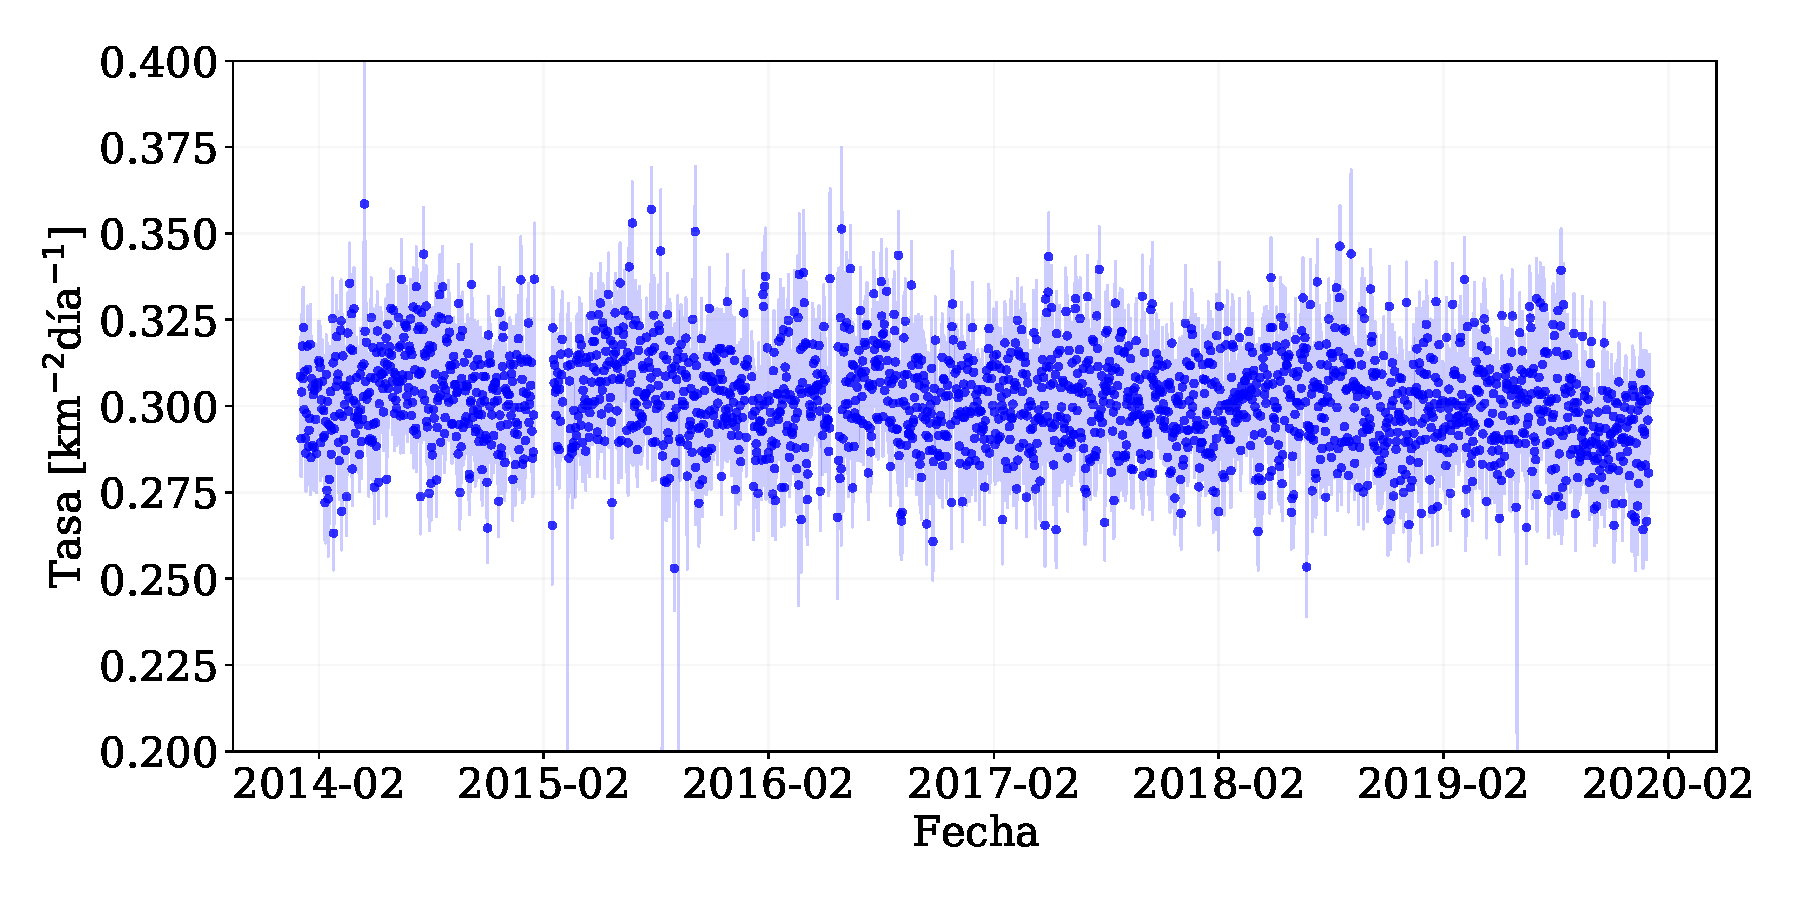
\includegraphics[width=0.5\textwidth]{tasa_eventos_corregido.pdf}
        \end{center}
        \caption{}
        \label{fig:corregido}
    \end{small}
\end{figure}

Dado que la señal S1000 y S38 de un evento en particular son proporcionales, asumiendo que la línea 12 es la señal S1000 sin corregir, puedo obtener la señal S38 sin la corrección del clima mediante:

\begin{align}
    S38_{sin\,corregir} = \frac{S1000_{sin\,corregir}}{S1000_{corregido}} S38_{corregido}
\end{align}
En el código de \verb|awk| se calcula mediante:
\begin{verbatim}
    (S38 sin corregir) = $12*$47/$37
\end{verbatim}

La prueba que se hizo para ver si la línea 12 está corregida o no, fue hacer el gráfico de tasa de eventos en función del tiempo en el rango cercano a 1 EeV -  2 EeV. Ya que se quire estudiar los efectos de la corrección del clima en la energía, los valores reportados no son confiables y se utilizan los valores de S38 que equivalen aproximadamente a  1 EeV y 2 EeV, estos valores son:
\begin{verbatim}
    1 EeV --- 5.36 VEM
    2 EeV --- 10.25 VEM
\end{verbatim}
Esta estimación se realizó con eventos del disparo estándar. Finalmente en la Fig.\ref{fig:nocorregido} se observa  una modulación anual, por lo que efectivamente la línea 12 es la señal S1000 sin corregir.

\begin{figure}[H]
    \begin{small}
        \begin{center}
            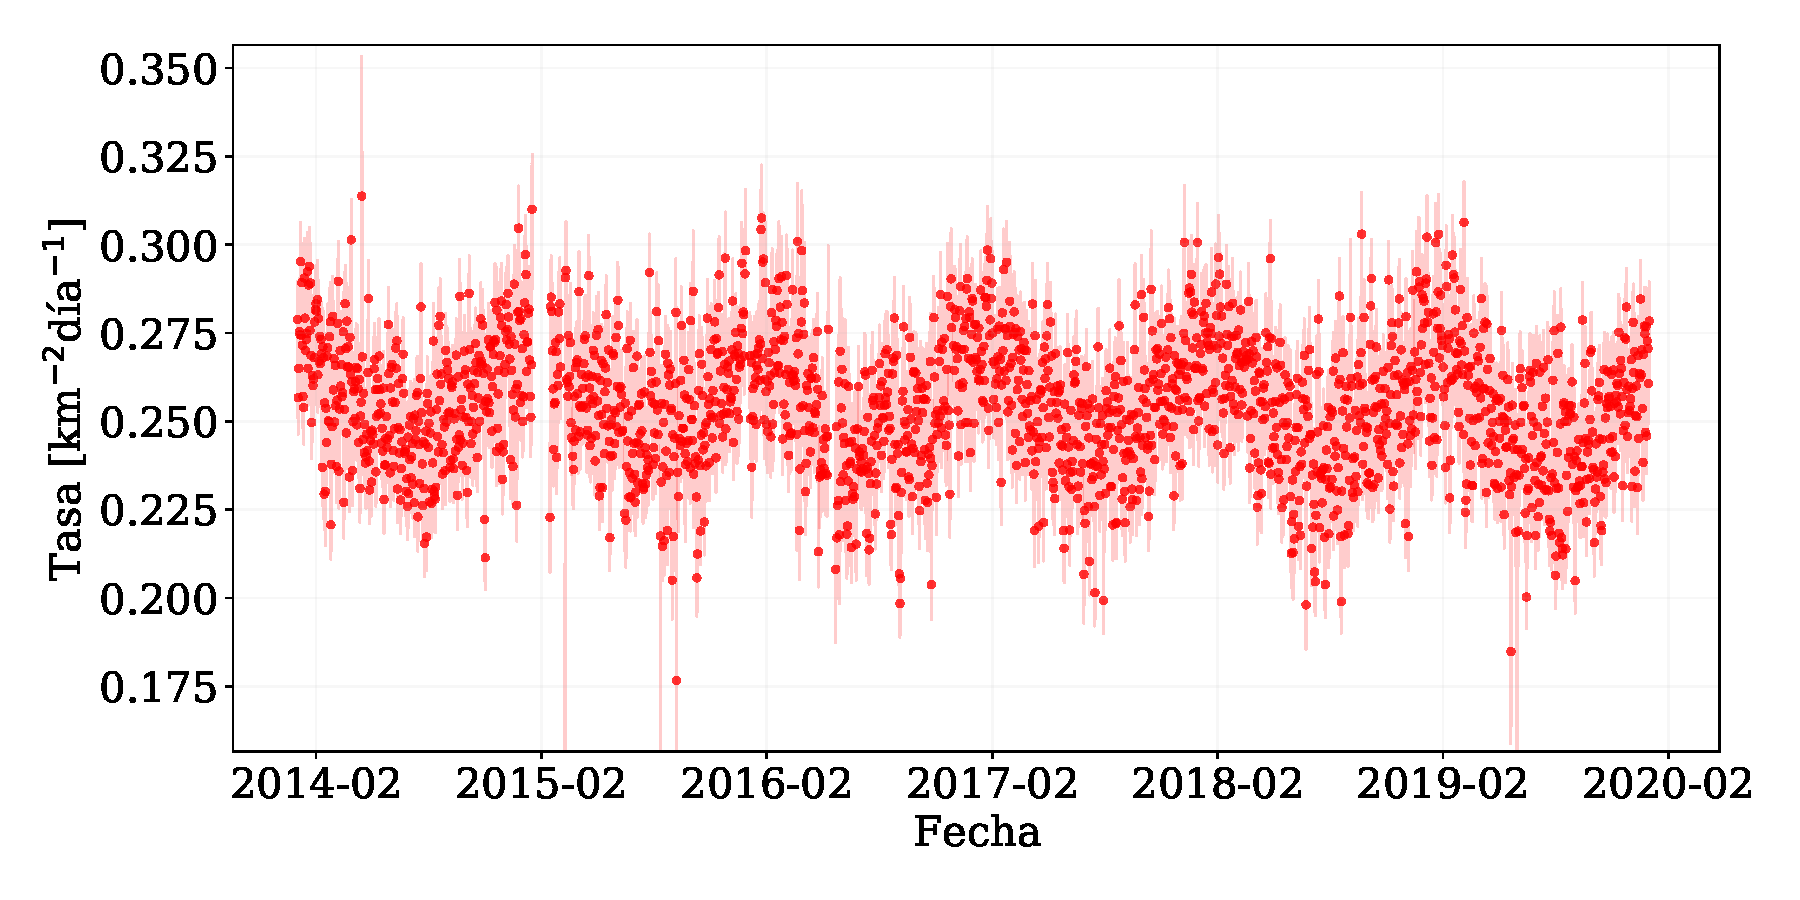
\includegraphics[width=0.5\textwidth]{tasa_eventos_sin_corregir.pdf}
        \end{center}
        \caption{}
        \label{fig:nocorregido}
    \end{small}
\end{figure}

\subsection{La reconstrucción}



\begin{enumerate}
    \item Se calculan nuevos parámetros del clima, filtrando con la señal de S38.
    \item Para reconstruir la energía  asociada a un evento, se aplica la nueva corrección del clima de la señal $S38_{sin\,correccion}$:
    \begin{verbatim}
        energy_corr = energy_reconstruction(S38*(S1000_raw/S1000), 
        p,  rho, rho_delay, the) 
    \end{verbatim}
    \item En la función \verb|energy_reconstruction|:
    \begin{verbatim}
        energy_reconstruction(S38, p, rho, rho_delay, the)
        {
            double d2r=M_PI/180.;
            double the2 = sin(the*d2r)*sin(the*d2r);

            factor =1.0 + alpha_p(the2)*(p-p0) 
                        + alpha_rho(the2)*(rho -  rho0) 
                        + beta_rho(the2)*(rhod - rho); 

            (nuevo S38) = S38/factor;

            return A*(nuevo S38)^B;
        }
    \end{verbatim}
    

\end{enumerate}


\end{document}
